\documentclass{beamer}
\usetheme{metropolis}

\usepackage[T1]{fontenc}
\usepackage[type1]{libertine}
\usepackage{amsmath}
\usepackage{caption}
\usepackage{bm}
\renewcommand{\ttdefault}{cmtt}
\usepackage[font=scriptsize]{caption}
\setbeamerfont{footnote}{size=\scriptsize}

\title{Observations of Low-altitude Arctic Cloud Properties at the Zeppelin Observatory}
\subtitle{A Quick Overview}
\author{Lawrence Oh, Sangjong Park, Joohong Kim}
\institute{Korea Polar Research Institute (KOPRI)}
\date{October 2022}

\begin{document}

\frame{\titlepage}

\begin{frame}
    \frametitle{Zeppelin Observatory}
    Ny-\r{A}lesund, Svalbard, Norway

    \begin{figure}
        \centering
        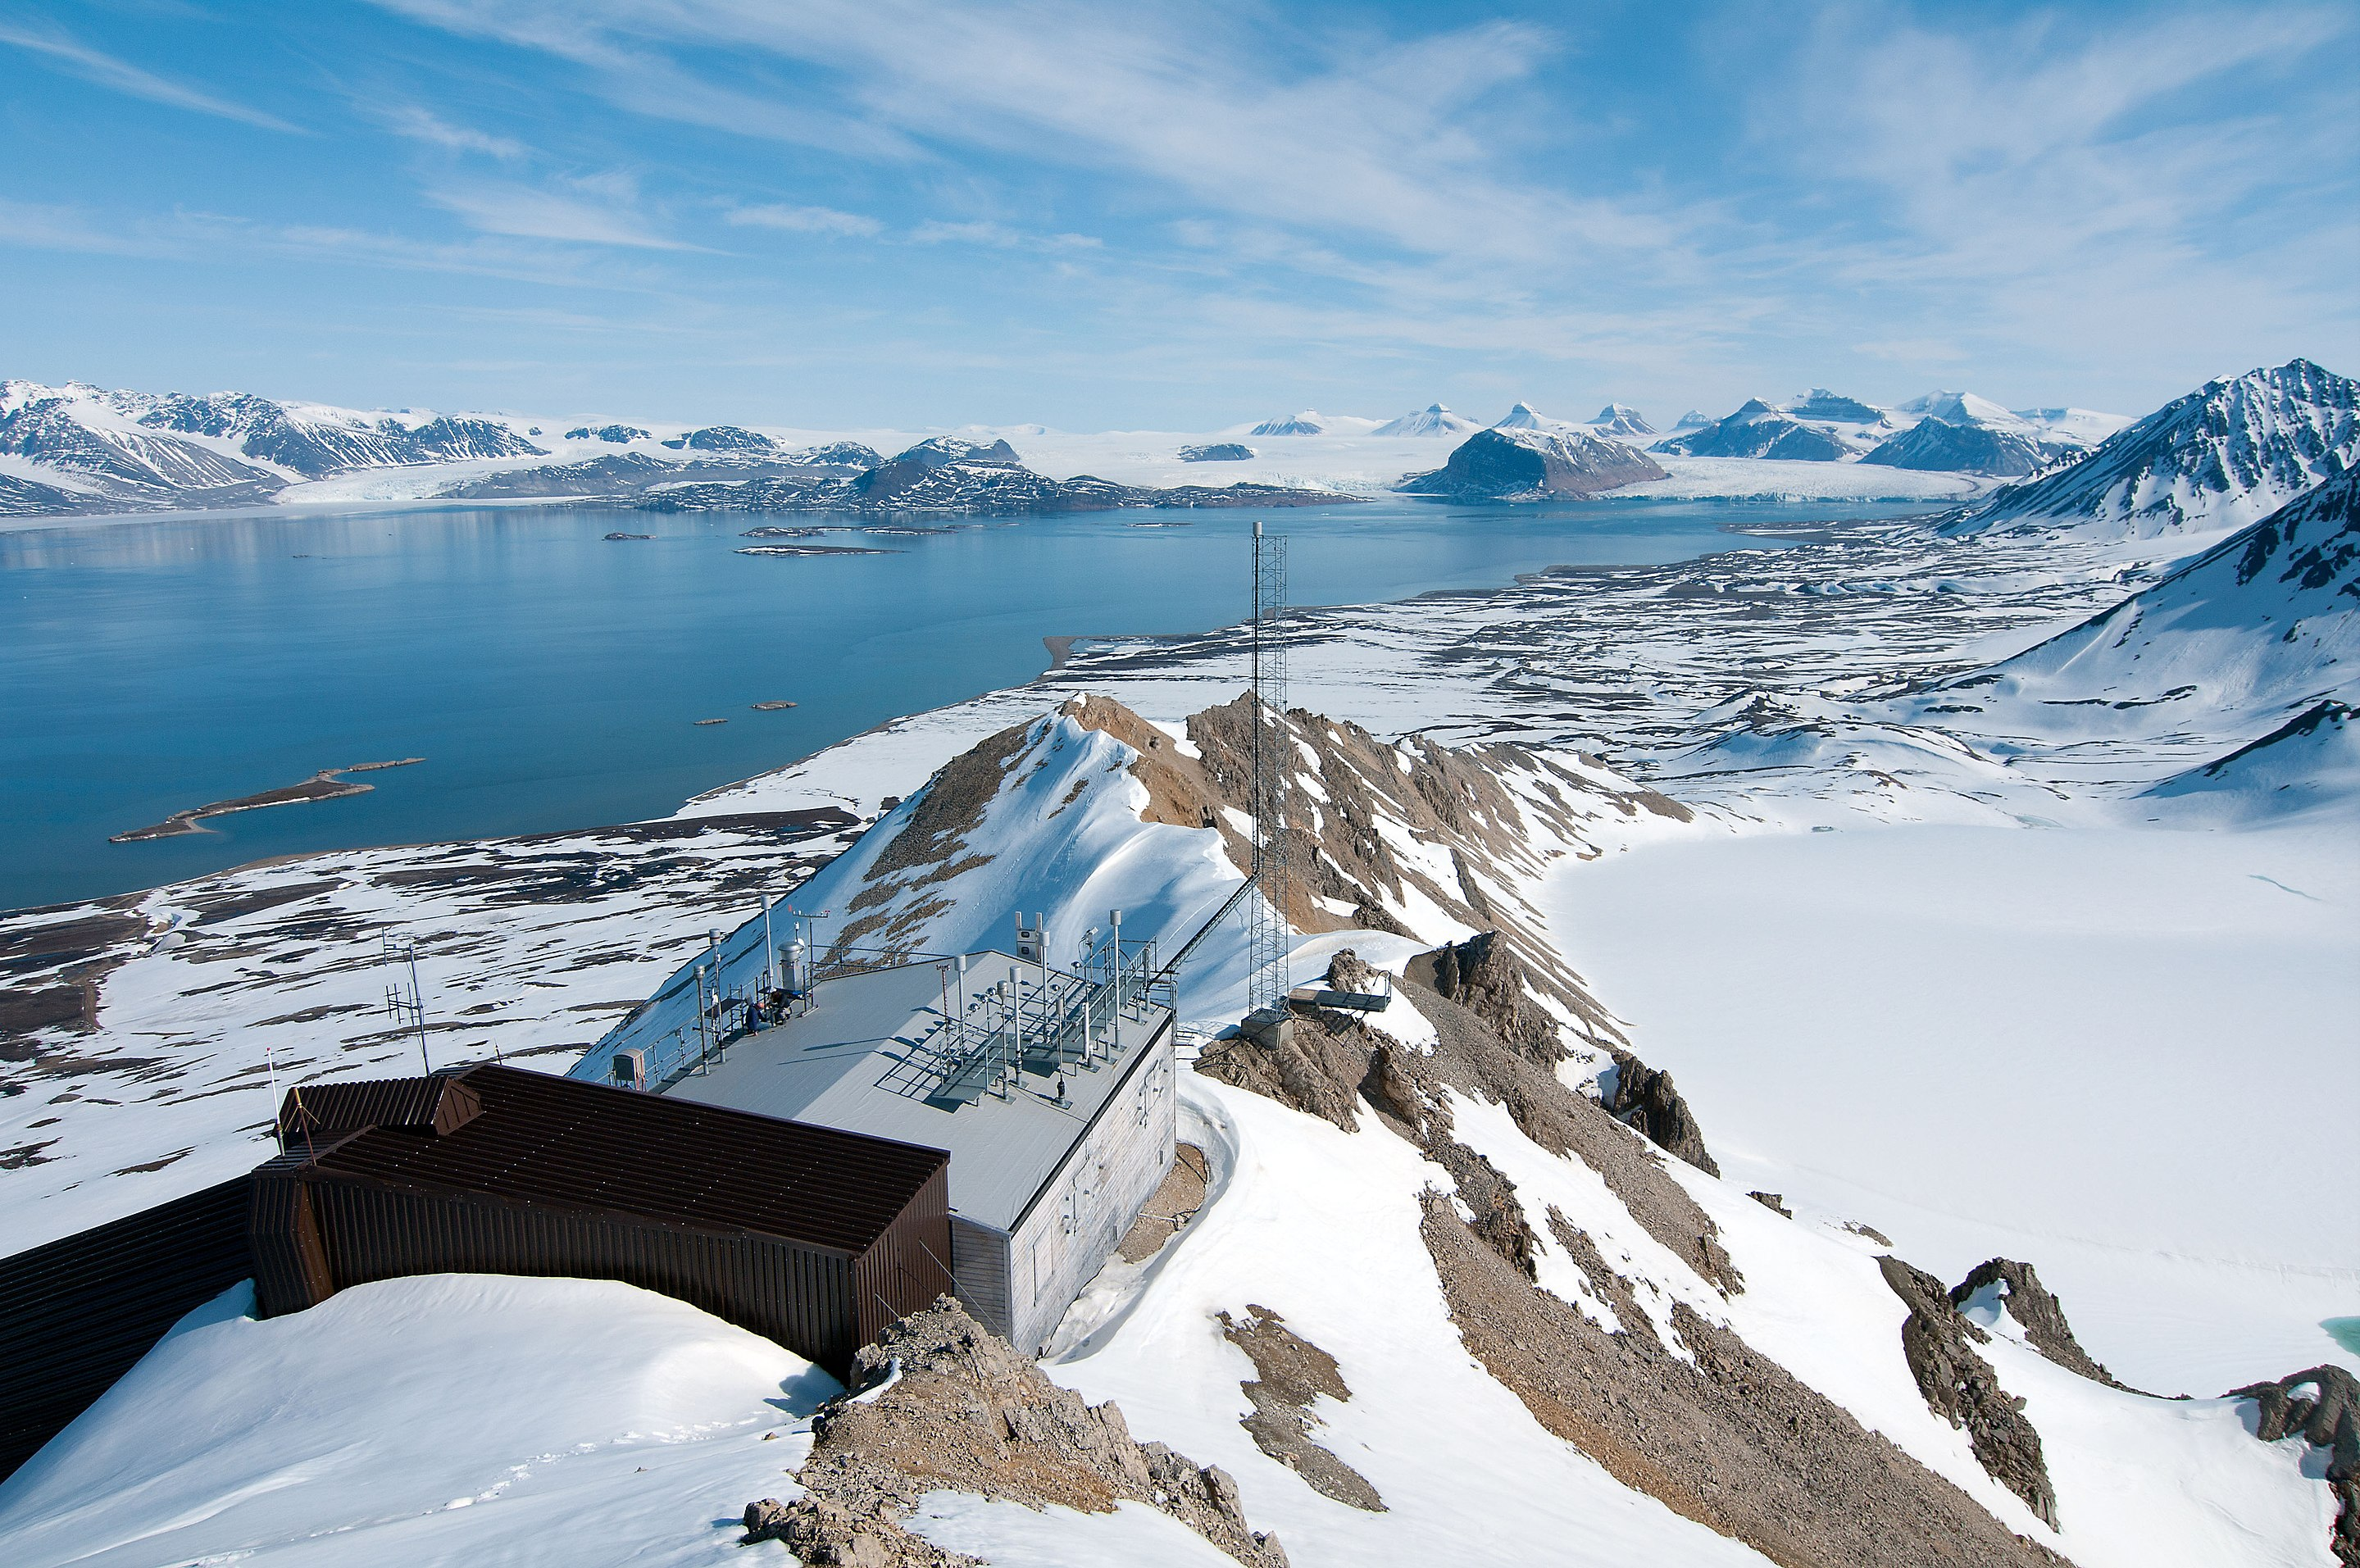
\includegraphics[width=0.8\textwidth]{img/zepp.jpeg}
        \caption{ An Overview of the Zeppelin Observatory }
    \end{figure}
\end{frame}

\begin{frame}
    \frametitle{Zeppelin Observatory}
    Two cloud droplet probes, CDP2 and BCPD

    \begin{figure}
        \centering
        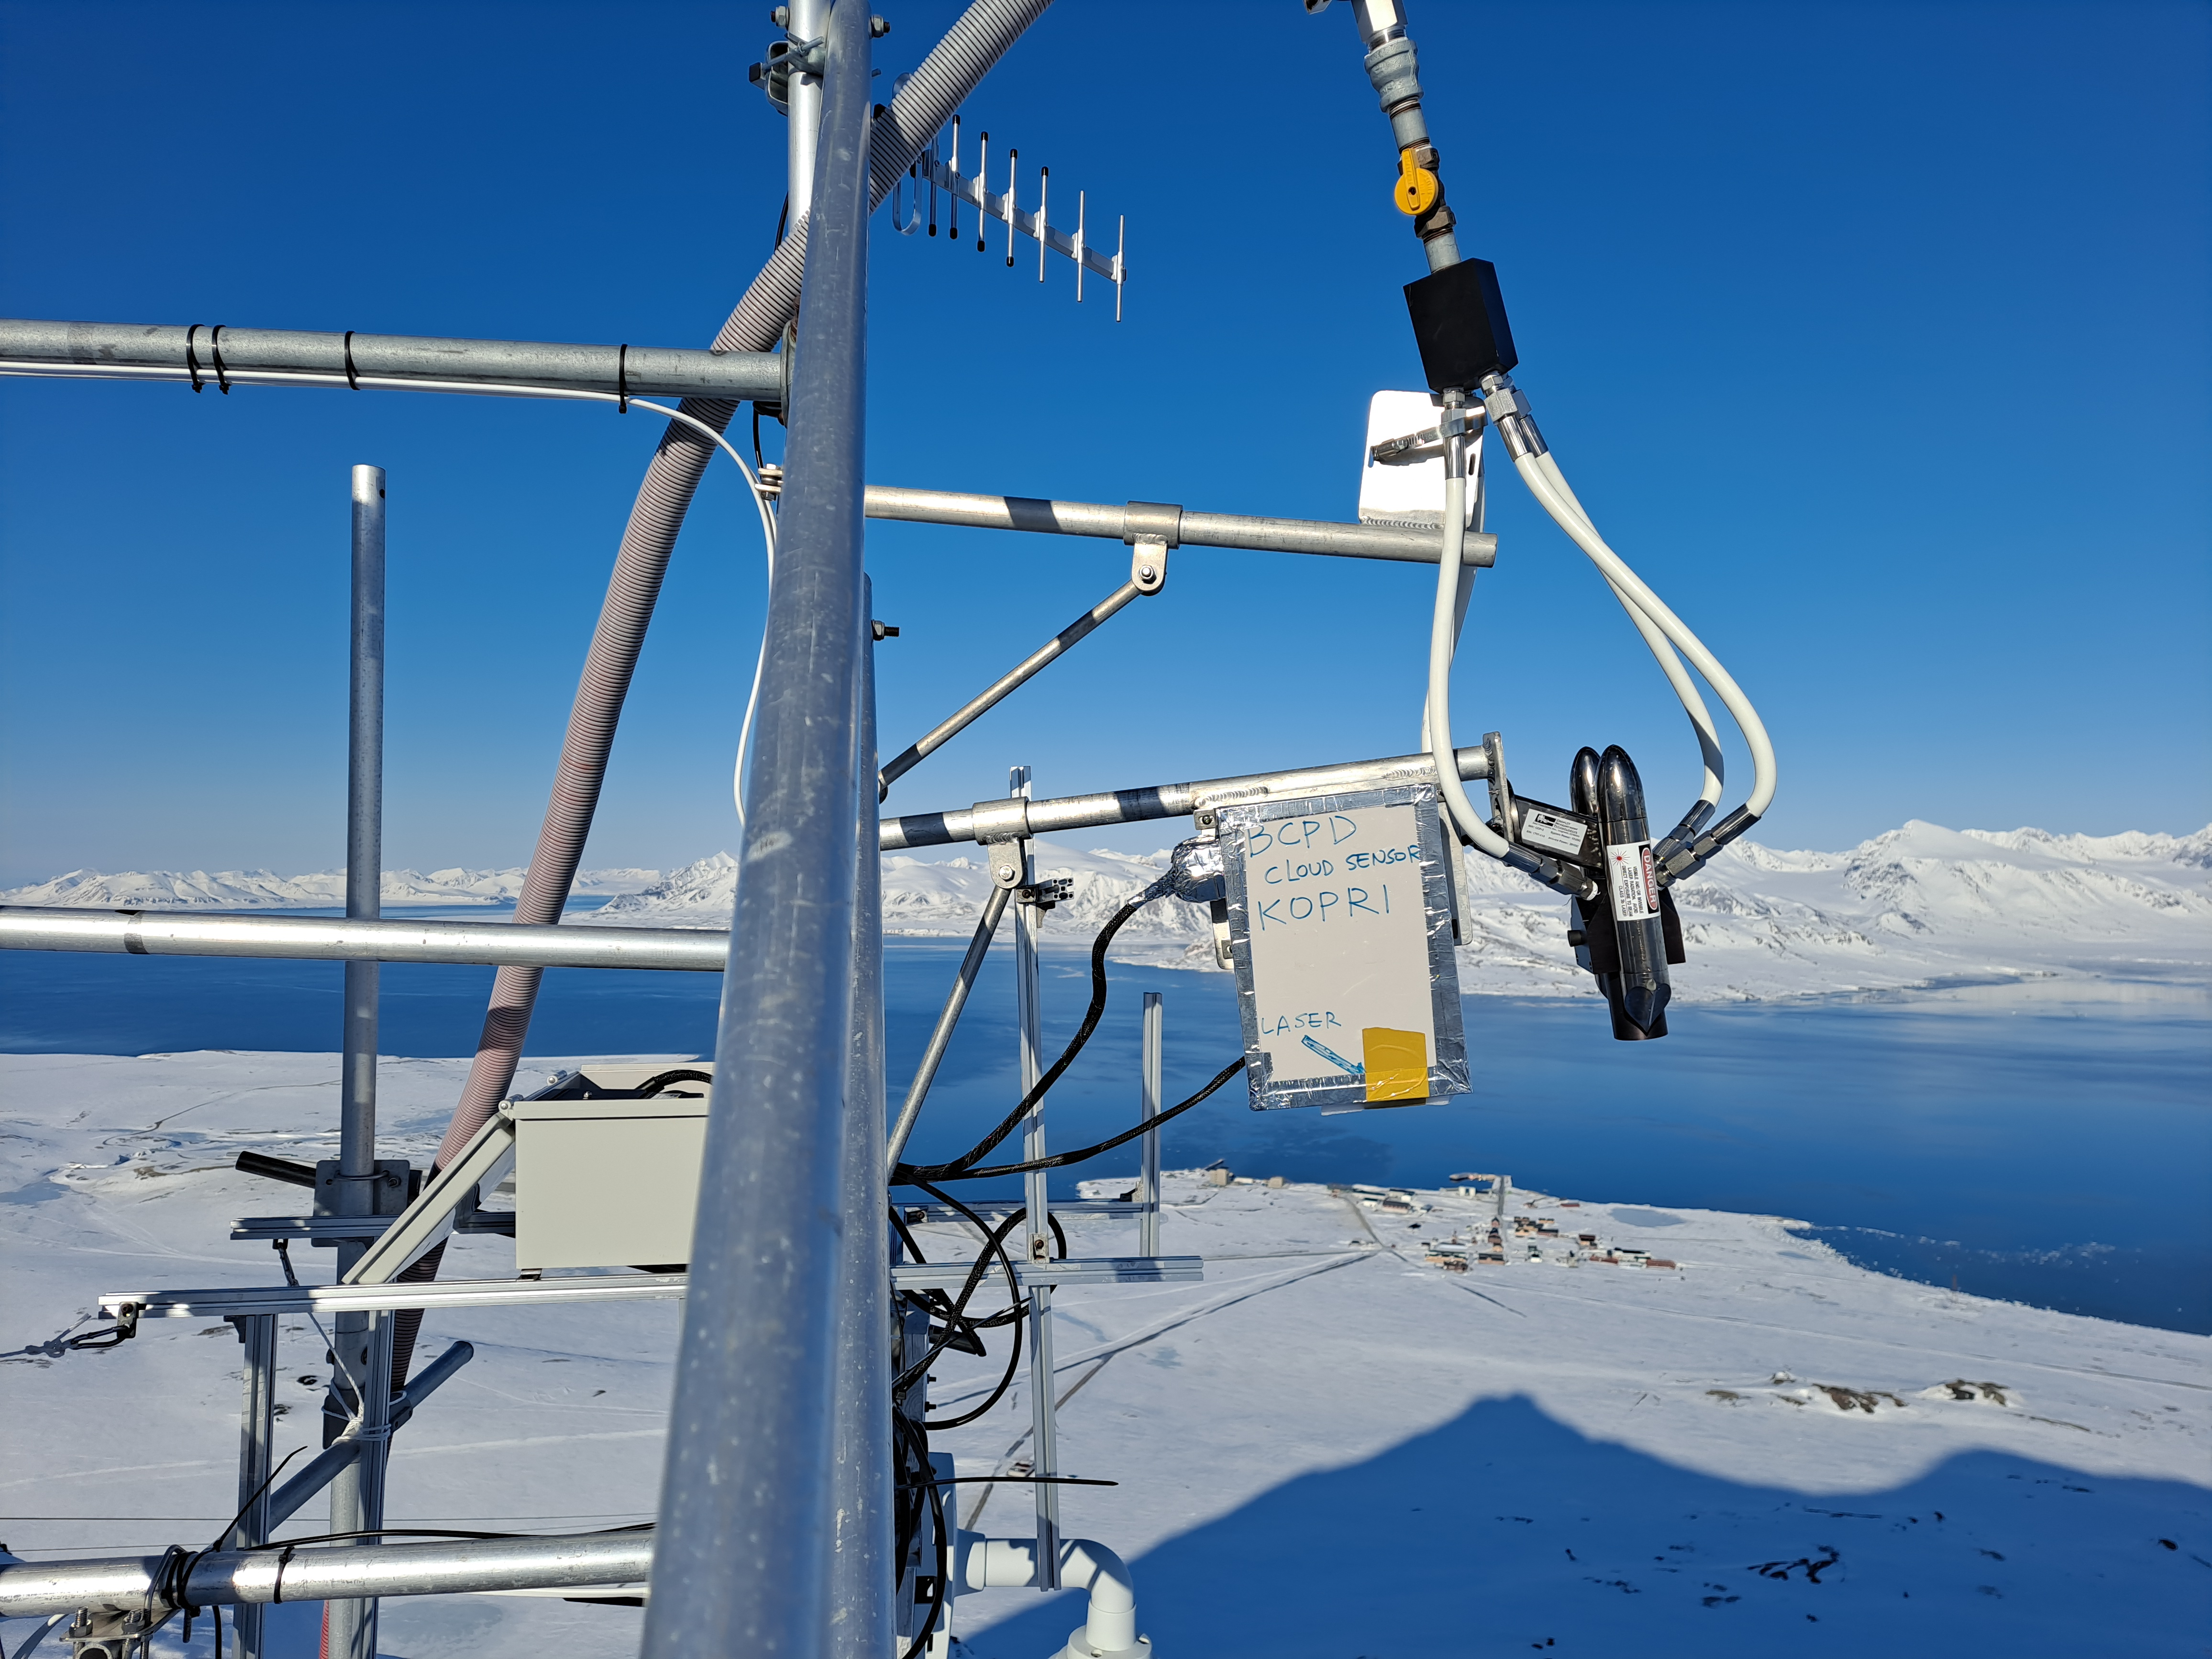
\includegraphics[width=0.75\textwidth]{img/zepp_cdp.jpg}
        \caption{ CDP2 (right) and BCPD (left), mounted at the Zeppelin Observatory }
    \end{figure}
\end{frame}

\begin{frame}
    \frametitle{Cloud Droplet Probe 2 (CDP2)}
    CDP2 is used to measure the cloud droplet size distribution from 2 $\mu$m to 50 $\mu$m, which is then used to calculate other cloud parameters

    \begin{figure}
        \centering
        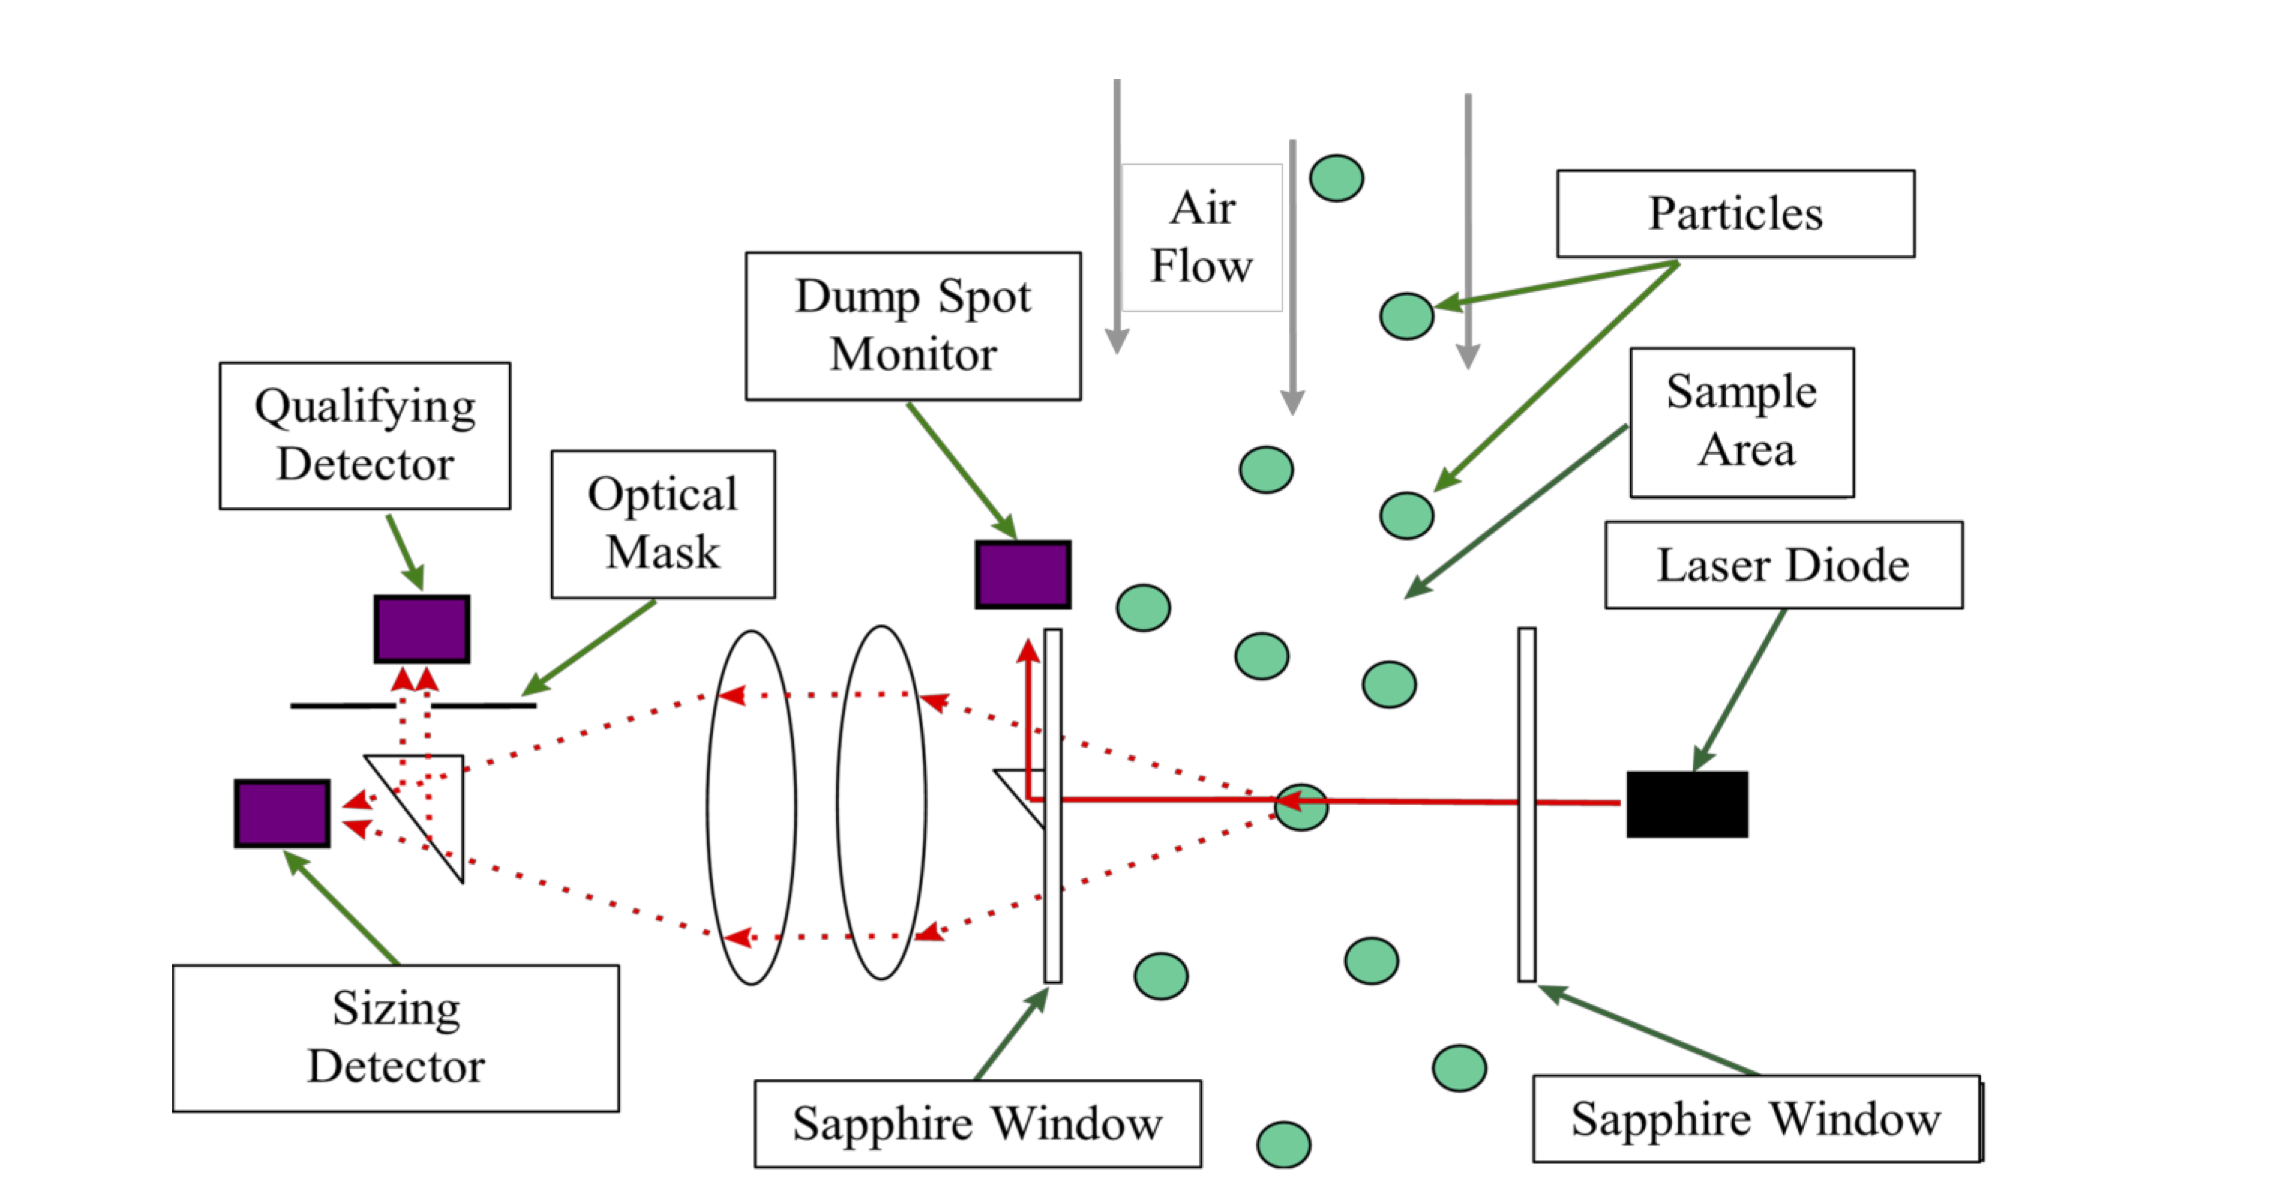
\includegraphics[width=0.8\textwidth]{img/cdp_op.png}
        \caption{ Operational Schematic Diagram for CDP2 }
    \end{figure}
\end{frame}

\begin{frame}
    \frametitle{Calculate True Air Speed}
    Because of the discrepancy between the default passing air speed (PAS) and the actual speed of the particles, one needs to estimate the latter based on average transit time:
    \begin{equation*}
         \mathrm{PAS}_\mathrm{True} \approx 150 \, [\mu \mathrm{m}] / \tau \, [\mu \mathrm{s}]
    \end{equation*}
    where $\tau$ stands for the average transit time measured by CDP2.\\~\
\end{frame}

\begin{frame}
    \frametitle{Calculate True Air Speed}
    Calculate LWC from the ground up:

    \begin{figure}
        \centering
        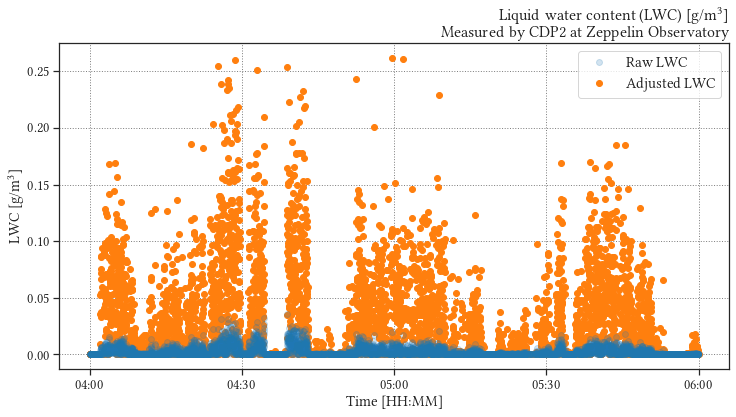
\includegraphics[width=0.8\textwidth]{img/pas.png}
        \caption{ Raw (blue) and adjusted (orange) time-series of LWC [g/m$^3$] on January 15th, 2018. }
    \end{figure}
\end{frame}

\begin{frame}
    \frametitle{Gassuain Process (GP) Regression}
    Consider a joint distribution of a set of observations $\mathbf{y}$ made at $\mathbf{x}$, and the function values $\mathbf{f}_*$ taken at test points $\mathbf{x}_*$, or
    \begin{equation*}
        p  \left(
        \begin{bmatrix}
            \mathbf{y} \\
            \mathbf{f}_*
        \end{bmatrix}
        \right) = \mathcal{N}
            \left(
            \begin{bmatrix}
                \bm{\mu} (\mathbf{x}) \\
                \bm{\mu} (\mathbf{x}_*)
            \end{bmatrix},
            	\begin{bmatrix}
            		\mathbf{K} (\mathbf{x}, \mathbf{x}) + \sigma^2 \mathbf{I}&
            		\mathbf{K} (\mathbf{x}, \mathbf{x}_*) \\
            		\mathbf{K} (\mathbf{x}_*, \mathbf{x}) &
            		\mathbf{K} (\mathbf{x}_*, \mathbf{x}_*)
            	\end{bmatrix}
            \right)
    \end{equation*}
    from which we can obtain the posterior distribution
    \begin{equation*}
        \bm{p}_* \triangleq p (\mathbf{f}_*) = \mathcal{N} (\mathbb{E}[\mathbf{f}_*], \mathbb{V} [\mathbf{f}_*])
    \end{equation*}
    that is fully specified by the posterior mean and variance
    \begin{align*}
        \mathbb{E}[\mathbf{f}_*] &= \bm{\mu}(\mathbf{x}_*) + 	\mathbf{K} (\mathbf{x}_*, \mathbf{x}) \left( \mathbf{K} (\mathbf{x}, \mathbf{x}) + \sigma^2 \mathbf{I} \right)^{-1} (\mathbf{y}(\mathbf{x}) - \bm{\mu}(\mathbf{x})) \\
        \mathbb{V} [\mathbf{f}_*] &= \mathbf{K} (\mathbf{x}_*, \mathbf{x}_*) - \mathbf{K} (\mathbf{x}_*, \mathbf{x}) \left( \mathbf{K} (\mathbf{x}, \mathbf{x}) + \sigma^2 \mathbf{I} \right)^{-1} \mathbf{K} (\mathbf{x}, \mathbf{x}_*)
    \end{align*}
    which defines the posterior distribution.
\end{frame}

\begin{frame}
    \frametitle{Gaussian Process (GP) Regression}
    The most widely used covariance function is the Square-Exponential (SE), defined as
    \begin{equation*}
        k_\mathrm{SE} = \exp \left( - \frac{(x - x')^2}{2 \lambda^2} \right)
    \end{equation*}
    where $\lambda$ is typically defined as a length scale, which is a hyper-parameter that determines how smooth the resulting process varies.
\end{frame}

\begin{frame}
    \frametitle{Re-sampling with Sparse GP Model}
    Using Gaussian Process Regression (GP) to re-sample time-series

    \begin{figure}
        \centering
        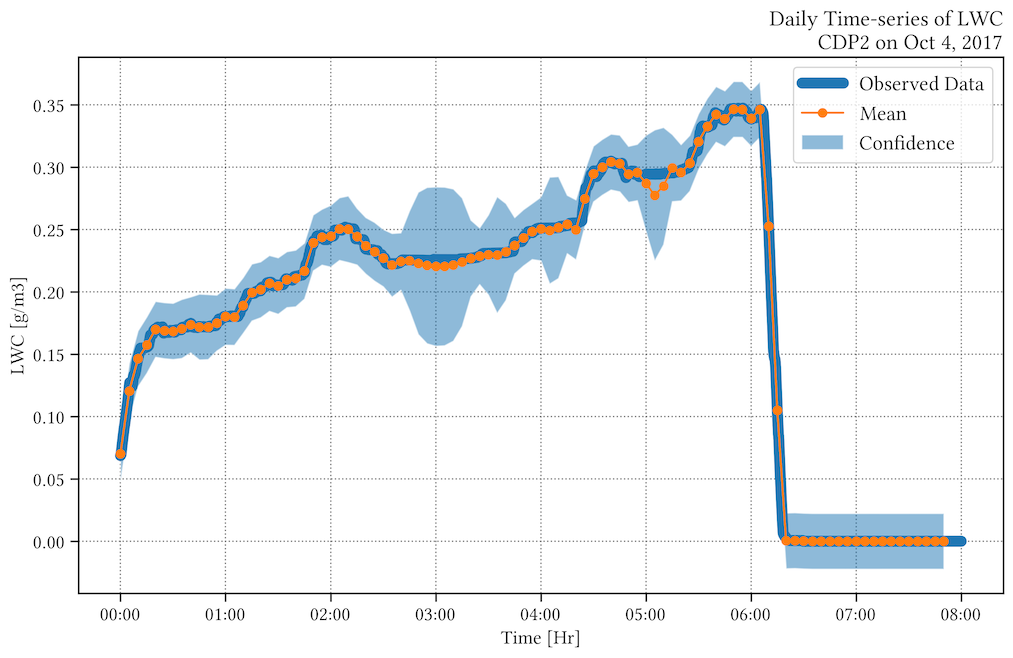
\includegraphics[width=0.8\textwidth]{img/cdp_gp02.png}
        \caption{Daily time-series of LWC [g/m$^3$] on January 15th, 2018.}
    \end{figure}
\end{frame}

\begin{frame}
    \frametitle{Comparison to Fog Monitor Measurements}
    \begin{figure}
        \centering
        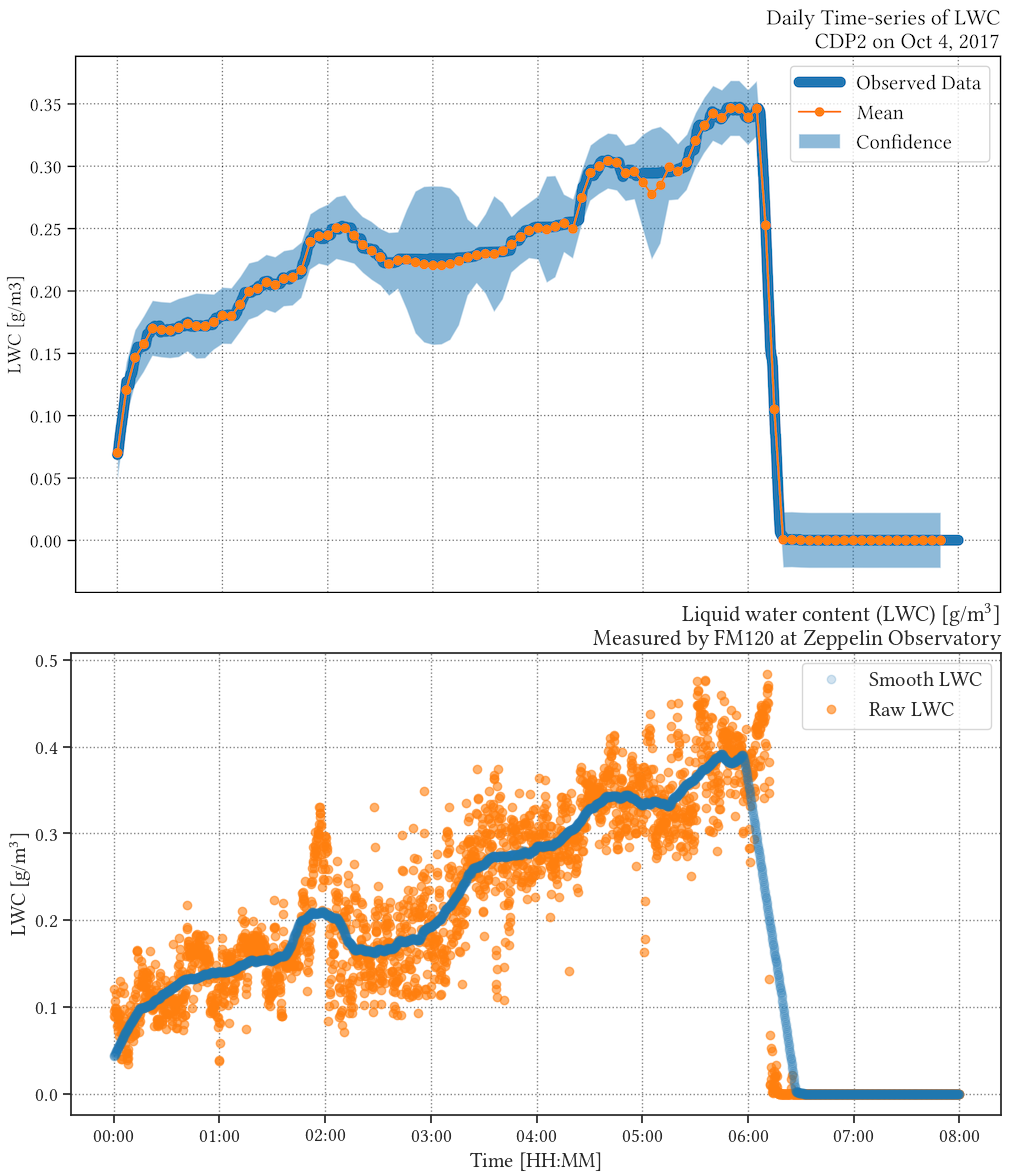
\includegraphics[width=0.65\textwidth]{img/comp.png}
        \caption{}
    \end{figure}
\end{frame}

\begin{frame}
    \frametitle{Measurements from Oct 4th, 2017}
    \begin{figure}
        \centering
        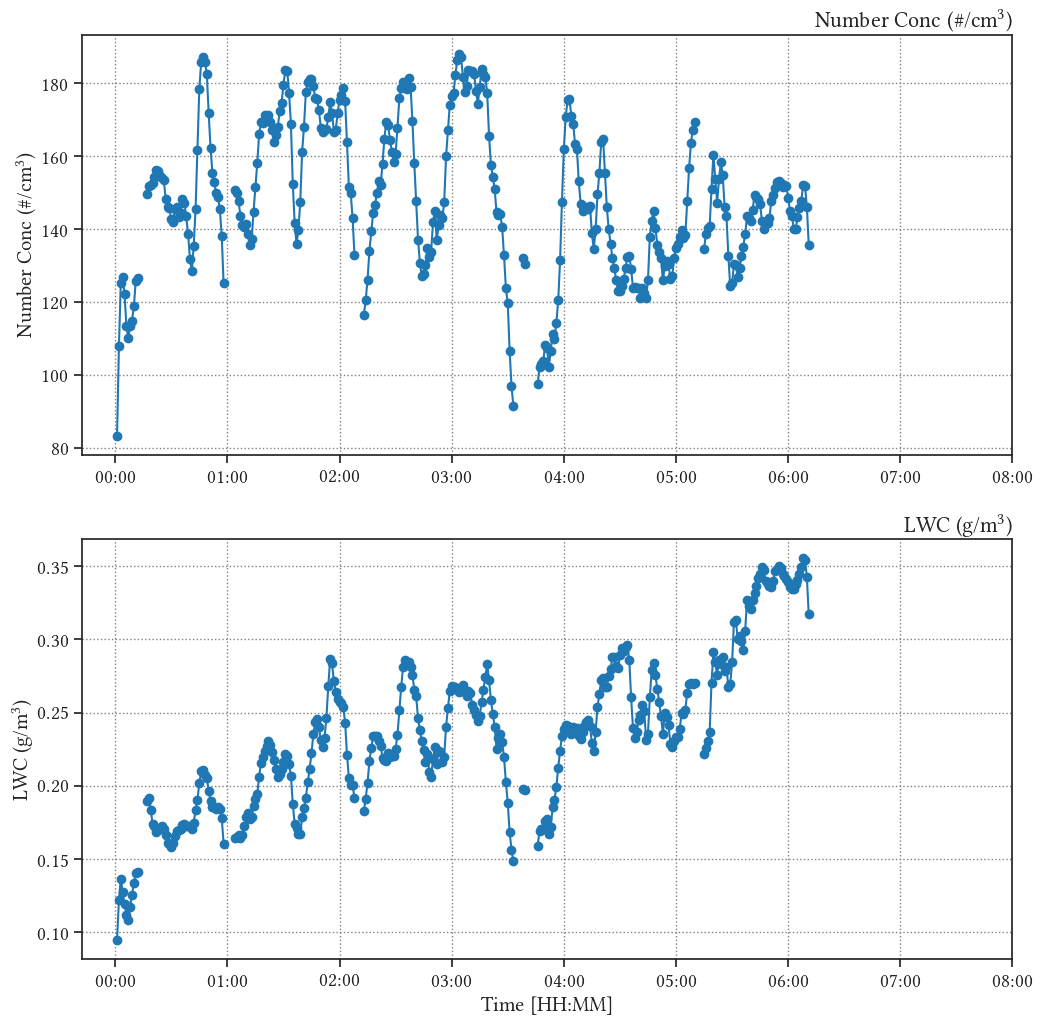
\includegraphics[width=0.7\textwidth]{img/cdp01.png}
        \caption{ NC and LWC Measured on Oct 4th, 2017 }
    \end{figure}
\end{frame}

\begin{frame}
    \frametitle{Measurements from Oct 4th, 2017}
    \begin{figure}
        \centering
        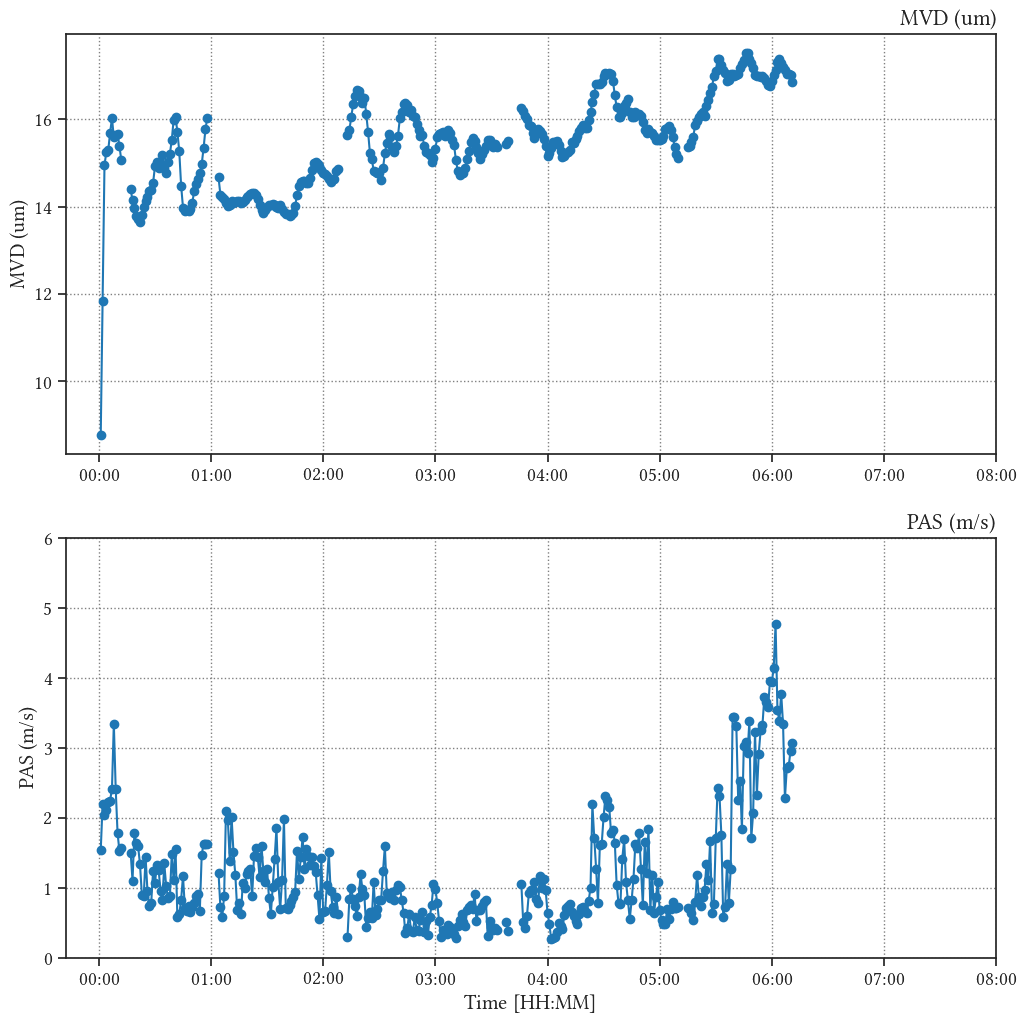
\includegraphics[width=0.7\textwidth]{img/cdp02.png}
        \caption{ MVD and PAS Measured on Oct 4th, 2017}
    \end{figure}
\end{frame}

\begin{frame}
    \frametitle{Measurements from Oct 4th, 2017}
    \begin{figure}
        \centering
        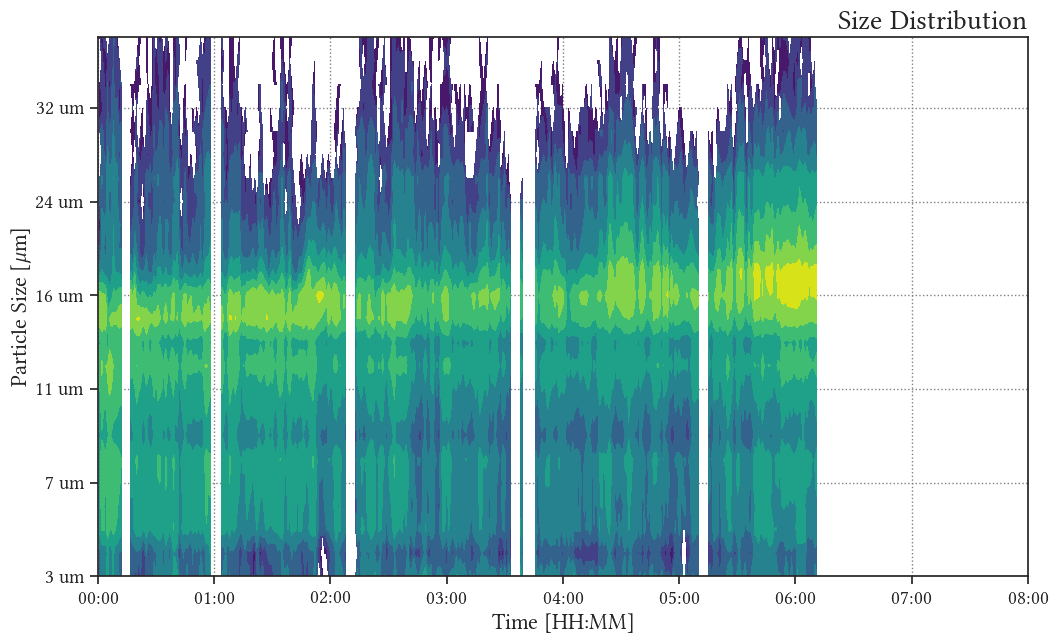
\includegraphics[width=0.75\textwidth]{img/size.png}
        \caption{ Size Distribution Measured on Oct 4th, 2017 }
    \end{figure}
\end{frame}

\begin{frame}
    \frametitle{Probe Uptime Between 2017 and 2022}
    \begin{figure}
        \centering
        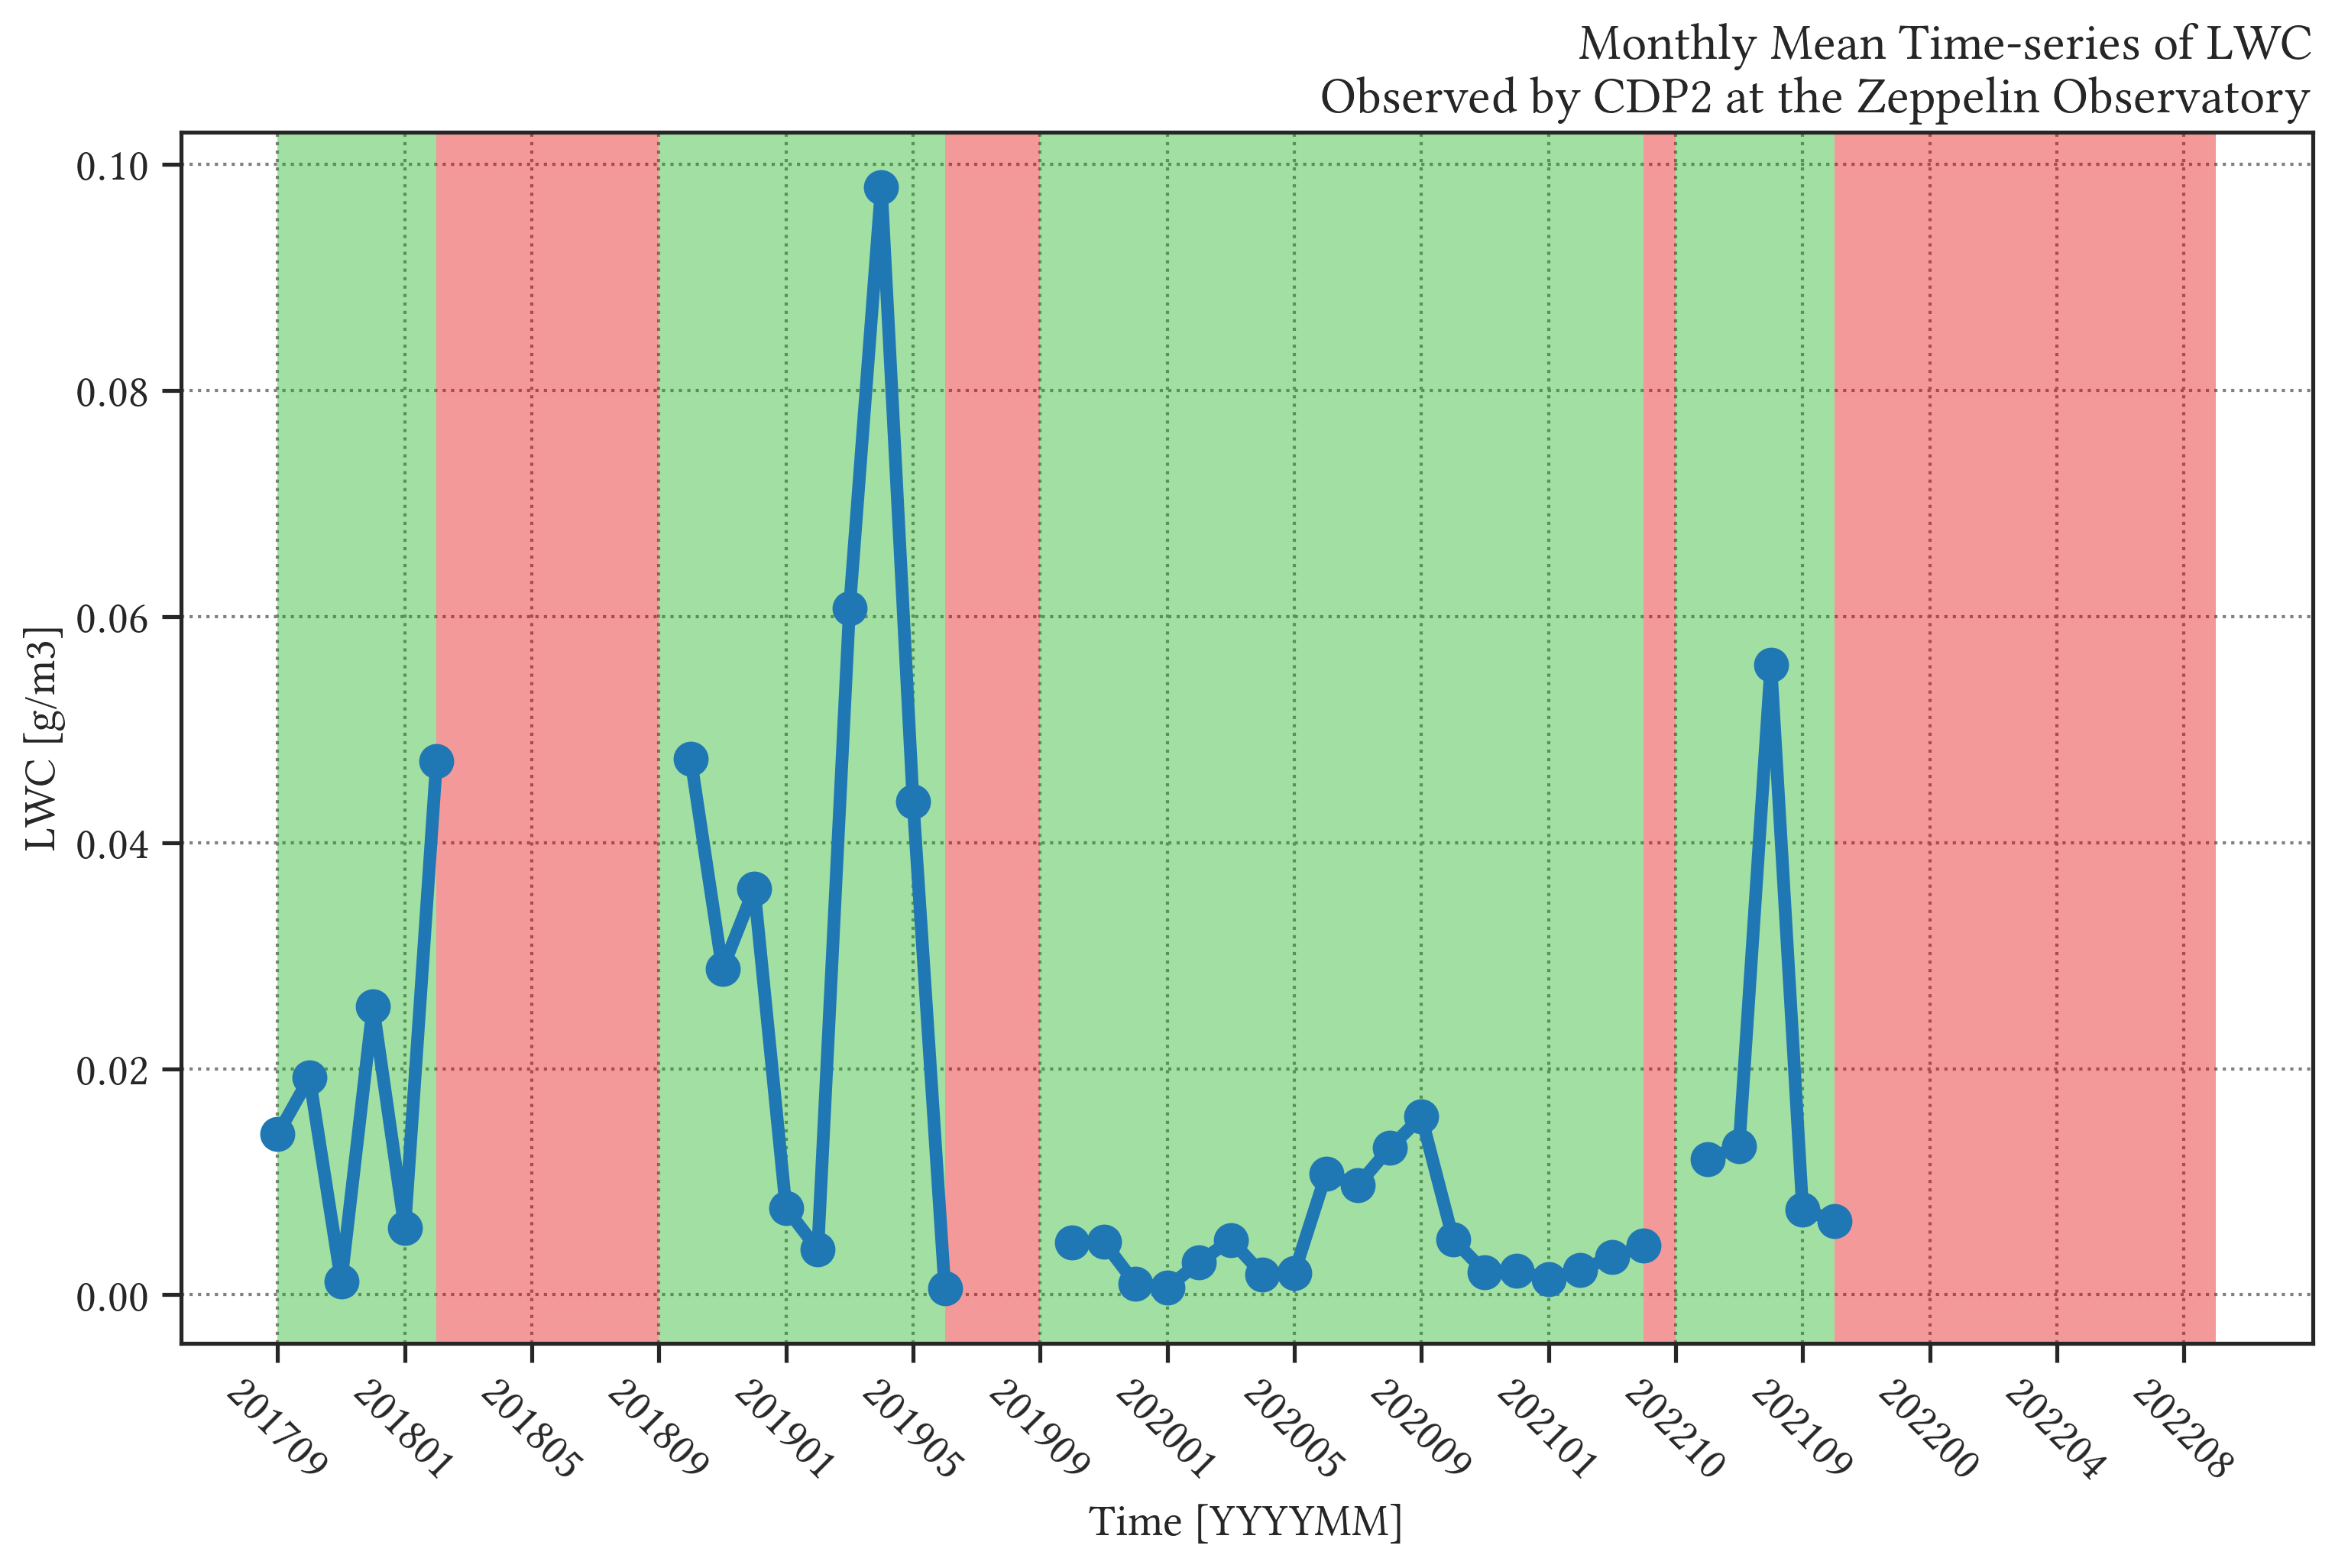
\includegraphics[width=0.75\textwidth]{img/monthly.png}
        \caption{ Opertional Period of CDP2 Since September 2017 }
    \end{figure}
\end{frame}

\begin{frame}
    \frametitle{Remarks}
    We have introduced a statistical method based on the Gaussian Process (GP) regrssion to analyze noisy time-series observations of low-altitude cloud properties from the cloud droplet probe (CDP2) and fog monitor (FM120). 
    
    The preliminary analysis shows that the two probes correspond well to each other, but a more quantitative analysis needs to be performed, especially during the warmer months.
\end{frame}

\end{document}